\subsection{Horizontal velocity (ice flow)}

\begin{figure}[H]
    \centering
    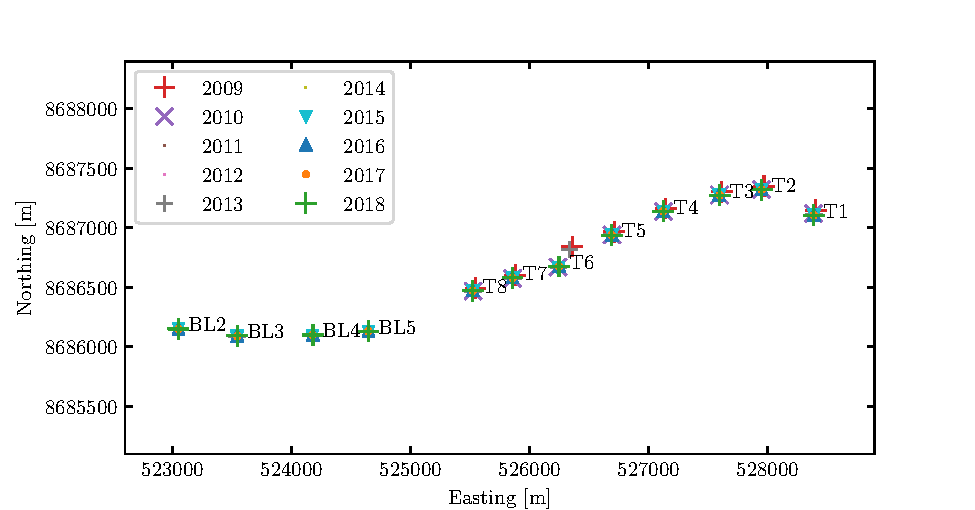
\includegraphics[width=\textwidth]{./figs/stakePositions.pdf}
    \caption{Positions of all stakes in the flow line on Blekumbreen and Tellbreen.
    The different markers distinguish the year of the measurement.}
    \label{GPS:fig:stakepos}
\end{figure}

Figure~\ref{GPS:fig:stakepos} shows the positions of the currently 12 different stake locations
on Blekumbreen and Tellbreen.
At those locations, a total of 26 measurements has been performed in 2018.
Additionally, all available data of the stake positions since 2009 is shown on the figure.\\
The coarse resolution of the figure shows a rough accordance of all of this years positions with the values 
of the last years.
The stakes spread over about 5 kilometers in east-west direction and 1.5 kilometers in north-south direction.

Figure~\ref{GPS:fig:T1_2d} shows all available data for one single stake (T1) in a higher resolution.\\
The measurement of the location of T1-2017 (green) has been performed two times
(Figs.~\ref{GPS:fig:T1-i_timeseries} and \ref{GPS:fig:T1-ii_timeseries})
in order to estimate the uncertainty
of the position.
The two positions differ by 19\,cm and match within their uncertainties.

Equation~\ref{GPS:eq:v} gives the realtion how the ice velocity $v_{year}$ has been calculated from the corrected stake positions in
Tab.~\ref{GPS:tab:os_tab}:
The distance between this years position and the position measured in 2017, 2016 or 2015 has been divided
by the passed time $t$ (1, 2 or 3 years).
$N_{year}$ and $E_{year}$ are the northing and easting of the year which has been used to calculate the distance to
this years position.
The positions of this year ($N_{year, 2018}$ and $E_{year, 2018}$) have been shifted by the respective distance
$\Delta_{\text{ref}, year}$ that ablation has
added to inclined stakes since the year $year$, as described in section~\ref{GPS:sec:Processing}.
Equation~\ref{GPS:eq:sv} shows how the error on $v_{year}$ has been obtained.

Table~\ref{GPS:tab:vel_tab} lists the calculated velocities for all stakes.
The direction of the movements can be seen on the detailed figures for each stake in the appendix.


\begin{figure}[H]
    \centering
    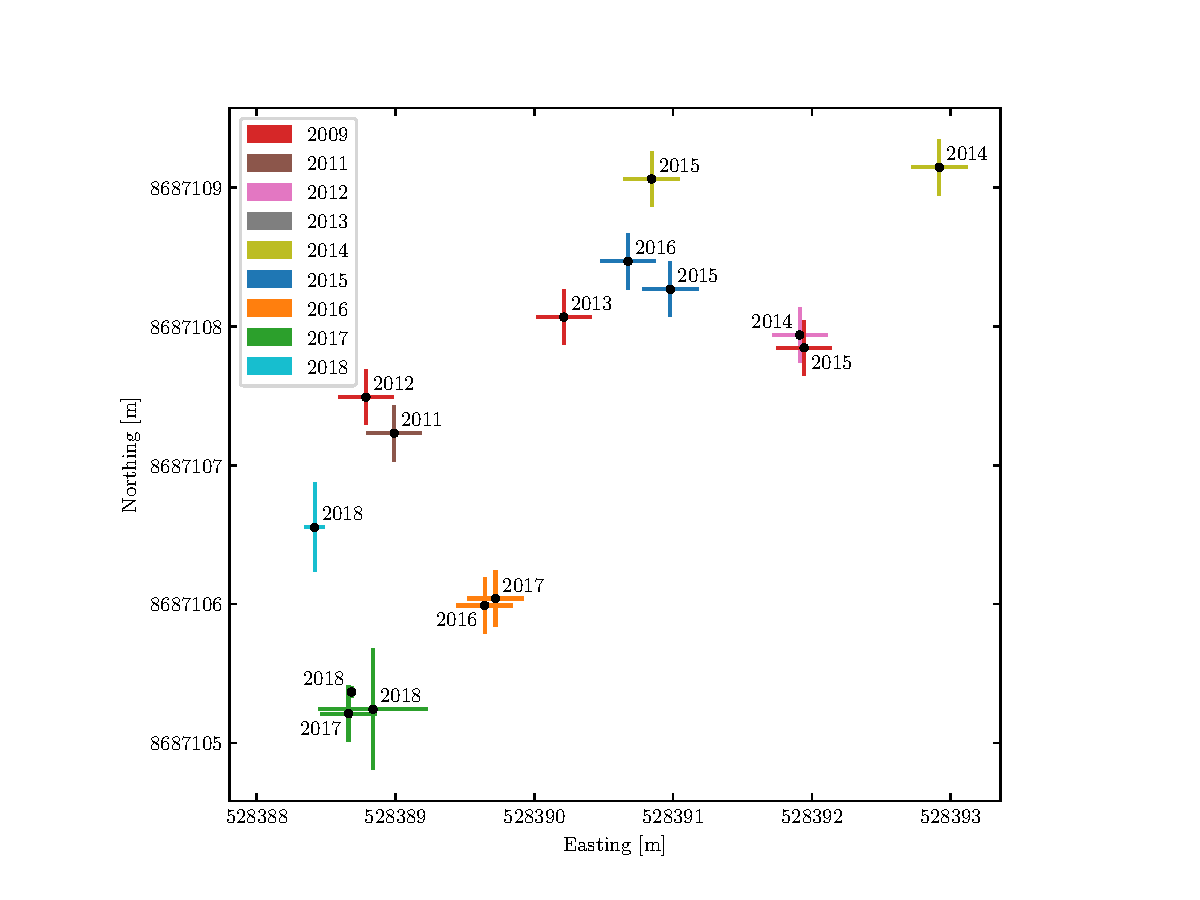
\includegraphics[width=\textwidth]{./figs/T1_2d.pdf}
    \caption{Measured positions at the location of stake T1 from 2011 to 2018.
    Different colors denote different stakes;
  	the year next to each stake position is the year of the measurement.
  	The measurements of 2018 have been corrected by the inclination of the stake and
  	the distance between the stake and the rover, therefore the coordinates refer to the intersection point
  	of stake and glacier surface.
    	At this location, a movement in south-east direction would be expected.
    	This is not identifiable using the data at hand.
 	Similar plots of the other 11 stake locations are situated in the appendix.}
    \label{GPS:fig:T1_2d}
\end{figure}


\begin{table}[H]
	\caption{Velocities of the stakes measured in 2018, calculated with equations~\ref{GPS:eq:v} and \ref{GPS:eq:sv}.
	The velocity $v_{2017}$ has been calculated using last years position.
	For inclined stakes, this position has been corrected for the horizontal displacement due to ablation.
	If available, corrected positions from 2016 and 2015 have also been used to obtain $v_{2016}$ and $v_{2015}$.
	To be able to assess the uncertainty of the velocities, four measurements have been performed twice.
	This is denoted by the suffices -i and -ii.}
	\centering
	\begin{tabular}{lcccccc}
\toprule
  Stake name & Velocity (2017) [m/a] & Velocity (2016) [m/a] & Velocity (2015) [m/a] \\
\midrule
    BL2-2016 &       0.26 $\pm$ 0.21 &       0.21 $\pm$ 0.20 &                     - \\
    BL3-2016 &       0.16 $\pm$ 0.20 &       0.21 $\pm$ 0.18 &                     - \\
  BL4-i-2016 &       0.07 $\pm$ 0.26 &       0.08 $\pm$ 0.25 &                     - \\
 BL4-ii-2016 &       0.11 $\pm$ 0.56 &       0.05 $\pm$ 0.48 &                     - \\
  BL5-i-2017 &       1.75 $\pm$ 0.18 &                     - &                     - \\
 BL5-ii-2017 &       1.74 $\pm$ 0.24 &                     - &                     - \\
   T1-i-2017 &       0.09 $\pm$ 0.11 &                     - &                     - \\
  T1-ii-2017 &       0.19 $\pm$ 0.43 &                     - &                     - \\
     T2-2016 &       0.60 $\pm$ 0.24 &       0.28 $\pm$ 0.20 &                     - \\
   T2-i-2017 &       0.23 $\pm$ 0.30 &                     - &                     - \\
  T2-ii-2017 &       0.53 $\pm$ 0.51 &                     - &                     - \\
     T3-2017 &       0.10 $\pm$ 0.12 &                     - &                     - \\
     T4-2016 &       0.13 $\pm$ 0.38 &       0.17 $\pm$ 0.37 &                     - \\
     T5-2016 &       0.30 $\pm$ 0.33 &       0.12 $\pm$ 0.22 &                     - \\
     T6-2016 &       0.79 $\pm$ 0.31 &       0.12 $\pm$ 0.19 &                     - \\
     T7-2015 &       0.26 $\pm$ 0.27 &       0.10 $\pm$ 0.15 &       0.08 $\pm$ 0.19 \\
     T7-2017 &       1.33 $\pm$ 0.16 &                     - &                     - \\
     T8-2017 &       0.20 $\pm$ 0.24 &                     - &                     - \\
\bottomrule
\end{tabular}

	\label{GPS:tab:vel_tab}
\end{table}

\begin{equation}
\label{GPS:eq:v}
v_{year} = \frac{\sqrt{(N_{year, 2018}-N_{year})^2+(E_{year, 2018} - E_{year})^2}}{t}
\end{equation}

\begin{equation}
\label{GPS:eq:sv}
\delta_{v_{year}} = \sqrt{\frac{
(\delta_{N_{year, 2018}}^2 + \delta_{N_{year}}^2) * (N_{year, 2018}-N_{year})^2 +
(\delta_{E_{year, 2018}}^2 + \delta_{E_{year}}^2) * (E_{year, 2018}-E_{year})^2}
{(N_{year, 2018} - N_{year})^2+ (E_{year, 2018} - E_{year})^2}}
\end{equation}


\subsection{Vertical velocity (mass balance)}

Besides the horizontal position, the GPS data also contain elevation.
An analysis of the change of elevation (the vertical velocity) of the stakes over the past years offers the possibility to determine the individual average mass balances.\\
We have been able to find elevation data from former groups for the last 7 years,
back until 2011.
Figures~\ref{GPS:fig:elev_ble} and \ref{GPS:fig:elev_tel} show this data,
together with the new data from 2018.
For most of the old data points, the uncertainties are not known.
Therefore there are no error bars shown on the plots.

Apart from a couple of outliers, the elevation of all stakes decreases quite linear.
Therefore linear fits of the elevation have been performed for all stakes individually.
The results of the fits are shown in Tables~\ref{GPS:tab:mbal_ble} and \ref{GPS:tab:mbal_tel}.\\
With the individual mass balances for each stake,
it is possible to calculate the mass balance gradients and the equilibrium line elevations of the two glaciers.
This is shown in Figs.~\ref{GPS:fig:elev_ble_mbg} and \ref{GPS:fig:elev_tel_mbg}.
The values on the y-axis (stake elevation) are mean values of all elevation measurements of the different years.

The linear fits yield the following results for the equilibrium lines (EL) and mass balance gradients~(MBG) on Blekumbreen and Tellbreen:
\begin{equation*}
\begin{split}
\text{EL}_\text{B} = 751 \pm 45\, \text{m} \qquad \text{MBG}_\text{B} = 5.1 \pm 1.0\, \text{mm/m}\\
\text{EL}_\text{T} = 757 \pm 56\, \text{m} \qquad \text{MBG}_\text{T} = 6.8 \pm 1.4\, \text{mm/m}
\end{split}
\end{equation*}


\begin{figure}[h]
    \centering
    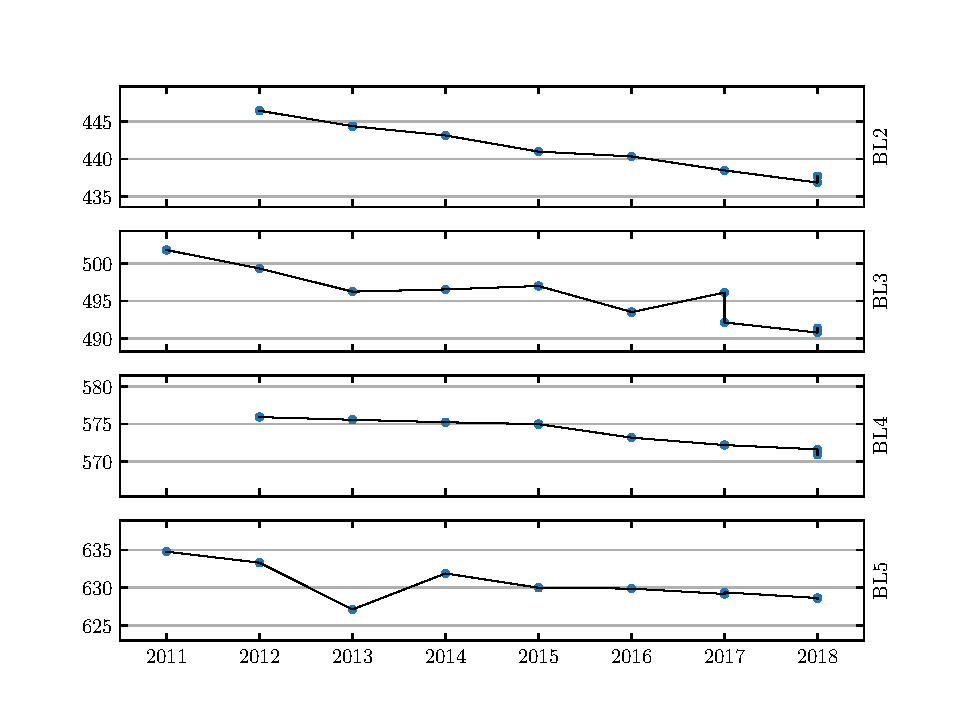
\includegraphics[width=\textwidth]{./figs/Elevation_Blekumbreen.pdf}
    \caption{GPS measured elevation of the stakes on Blekumbreen from 2011 until 2018 (blue dots).
    Linear fits (red line) of the data have been performed to calculate the individual mass balances~$b$.}
    \label{GPS:fig:elev_ble}
\end{figure}


\begin{figure}[h]
    \centering
    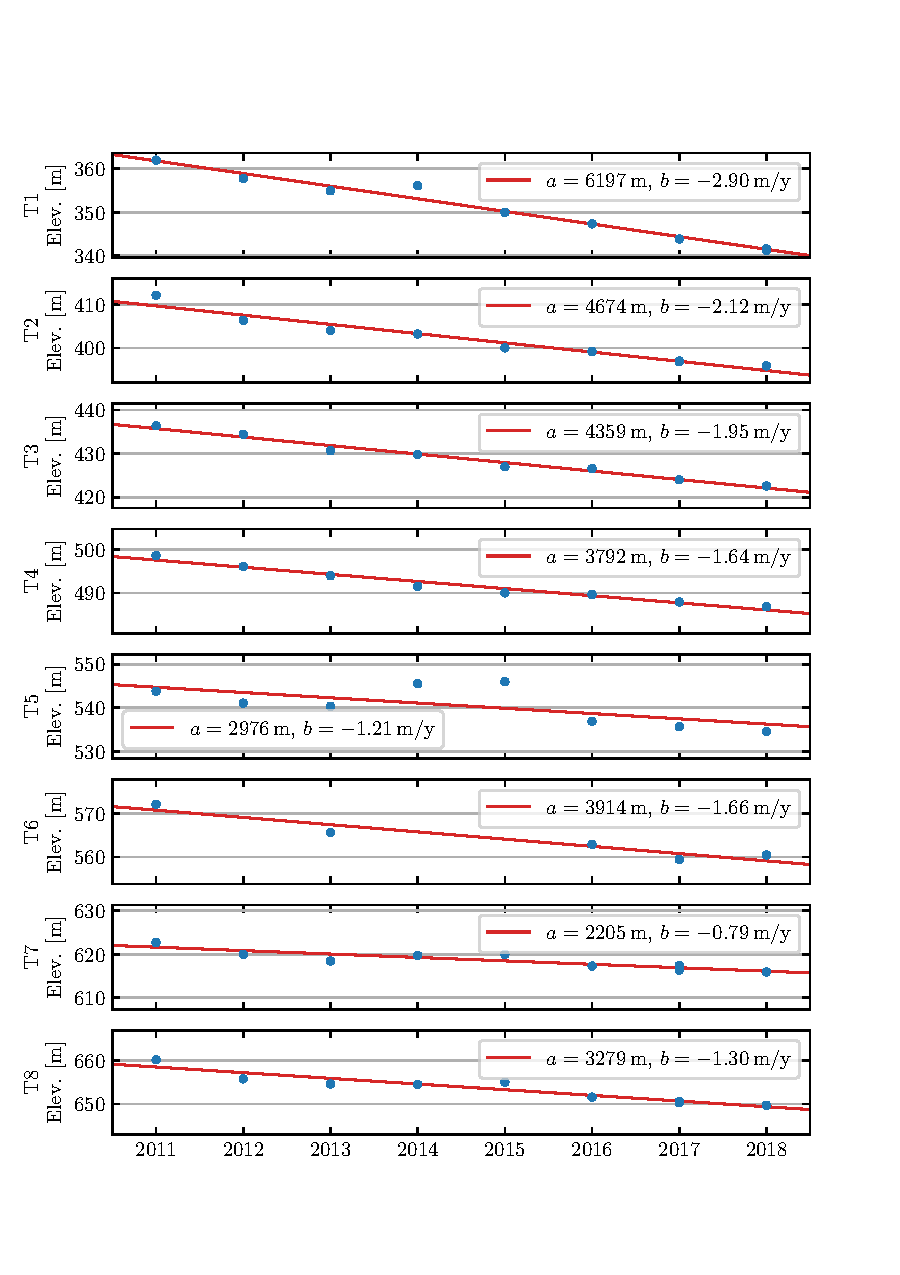
\includegraphics[width=\textwidth]{./figs/Elevation_Tellbreen.pdf}
    \caption{GPS measured elevation of the stakes on Tellbreen from 2011 until 2018 (blue dots).
    Linear fits (red line) with $y = a + x*b$ have been performed to calculate the individual mass balances~$b$.}
    \label{GPS:fig:elev_tel}
\end{figure}

\begin{table}[h]
	\caption{Mass balance as result of the elevation fits from Fig.~\ref{GPS:fig:elev_ble} and
	mean values of the elevation measurements for all stakes on Blekumbreen.
    The data in the table is plotted in Fig.~\ref{GPS:fig:elev_ble_mbg}.}
	\centering
	\begin{tabular}{lcc}
\toprule
Stake name & Elevation [m] &  Mass balance [m] \\
\midrule
       BL2 &         441.7 &  -1.45 $\pm$ 0.08 \\
       BL3 &         495.7 &  -1.44 $\pm$ 0.16 \\
       BL4 &         574.0 &  -0.85 $\pm$ 0.11 \\
       BL5 &         630.3 &  -0.65 $\pm$ 0.24 \\
\bottomrule
\end{tabular}

	\label{GPS:tab:mbal_ble}
\end{table}

\begin{table}[h]
	\caption{Mass balance as result of the elevation fits from Fig.~\ref{GPS:fig:elev_tel} and
	mean values of the elevation measurements for all stakes on Tellbreen.
    The data in the table is plotted in Fig.~\ref{GPS:fig:elev_tel_mbg}.}
	\centering
	\begin{tabular}{lcc}
\toprule
Stake name & Elevation [m] &  Mass balance [m] \\
\midrule
        T1 &         349.4 &  -2.90 $\pm$ 0.15 \\
        T2 &         401.4 &  -2.12 $\pm$ 0.17 \\
        T3 &         428.9 &  -1.95 $\pm$ 0.12 \\
        T4 &         491.8 &  -1.64 $\pm$ 0.13 \\
        T5 &         540.5 &  -1.21 $\pm$ 0.55 \\
        T6 &         564.1 &  -1.66 $\pm$ 0.30 \\
        T7 &         618.7 &  -0.79 $\pm$ 0.15 \\
        T8 &         653.6 &  -1.30 $\pm$ 0.17 \\
\bottomrule
\end{tabular}

	\label{GPS:tab:mbal_tel}
\end{table}

\begin{figure}[H]
    \centering
    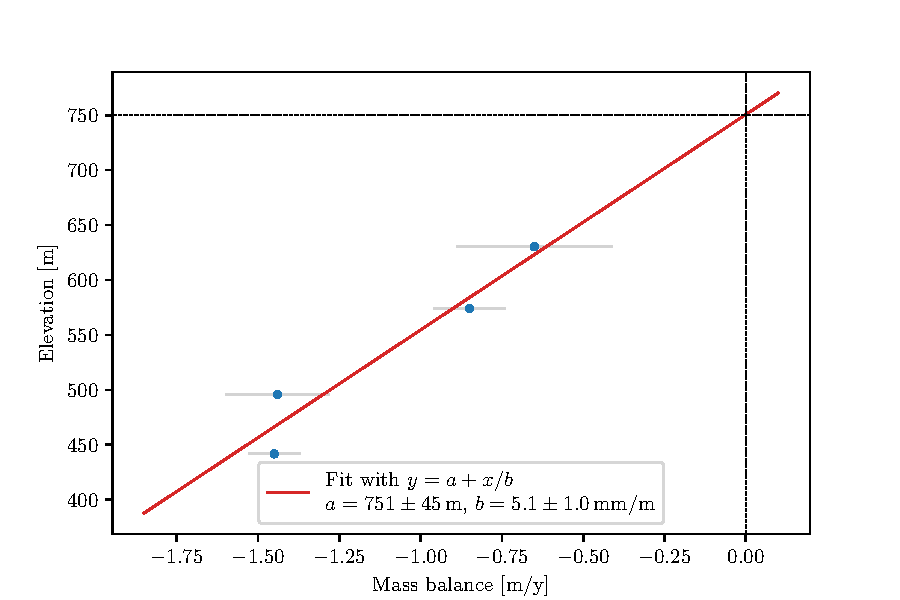
\includegraphics[width=\textwidth]{./figs/Elevation_Blekumbreen_mbg.pdf}
    \caption{Mass balances of the stakes on Blekumbreen as a function of stake elevation and linear fit of the points to obtain
    the equilibrium line elevation $a$ and the mass balance gradient $b$.}
    \label{GPS:fig:elev_ble_mbg}
\end{figure}


\begin{figure}[H]
    \centering
    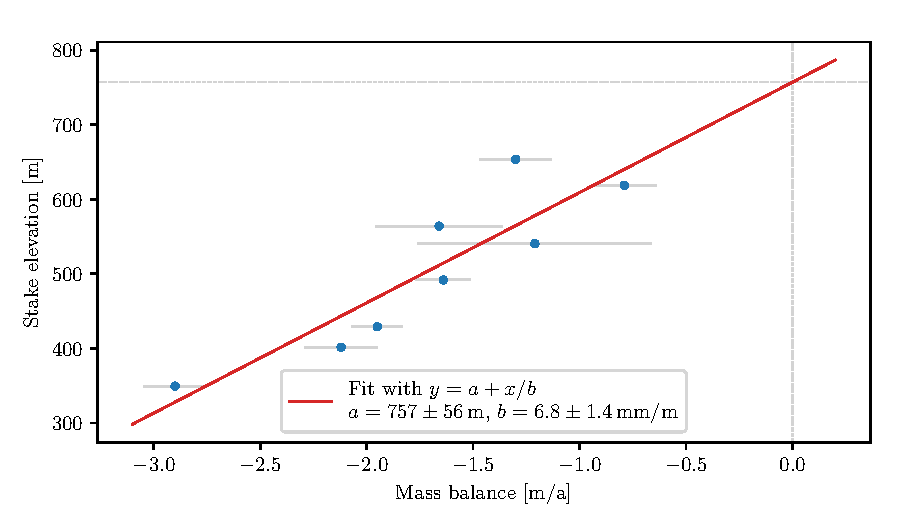
\includegraphics[width=\textwidth]{./figs/Elevation_Tellbreen_mbg.pdf}
    \caption{Mass balances of the stakes on Tellbreen as a function of stake elevation and linear fit of the points to obtain
    the equilibrium line elevation $a$ and the mass balance gradient $b$.}
    \label{GPS:fig:elev_tel_mbg}
\end{figure}

\subsection{Theoretical surface velocity}
% Different tables for different values of B(T = 0,-5,-10,-15), \alpha = 5,6,7 and H (from the ice-radar scans) = 1 (minimal value — minimum was at 3), 33.4 (average value), 82,3 (maximum)
Based on the shallow ice approximation is is possible to calculate a theoretical surface velocity for the glaciers we did our measurements on.
To make the calculation (see \ref{GPS:eq:sia}) the variables slope angle, ice velocity and ice thickness has to be choosen. 
The ice density is assumed as 917 kg/m$^3$ and the gravitational acceleration as 9.81  m/s$^2$.
The values for the ice viscosity are displayed in table \ref{GPS:tab:iceviscosities}.
It is not possible to determine the exact ice temperature.
Because of this, the calculation is done for viscosities for differnt ice temperatures $T$.

\begin{table}[H]
\centering
\begin{tabular}{lcccc}
\toprule
Temperature [$^\circ$C] & 0 & -5 & -10 & -15 \\
\midrule
Ice viscosity $\left[ P / \text{a}^{-3} \right]$ & $5,52 \cdot 10^7$ & $8,63 \cdot 10^7$ & $1.28 \cdot 10^8$ & $1.52 \cdot 10^8$\\
\bottomrule
\end{tabular}
\caption{Ice viscosities for different ice temperatures $T = \{0,-5,-10,-15\}$}
\label{GPS:tab:iceviscosities}
\end{table}

The theoretical velocity is mainly influenced by the ice thickness (see tables \ref{GPS:tab:theorytable5}, \ref{GPS:tab:theorytable6} and \ref{GPS:tab:theorytable7} ).
For the mean thickness the theoretical surface velocity of ice has the order of magnitude of centimeters. 
The small velocity value corresponds with the measured velocities (compare \ref{GPS:tab:vel_tab}). 

\begin{table}[H]
    \centering
    	\caption{Theoretical surface velocity $u_\circledS\,\left[m / \text{a} \right]$, $\alpha = 5$}
	\begin{tabular}{lccc}
	\toprule
	$\alpha=5$ & $H_{min} = 1$ & $H_{avg}=33.4$ & $H_{max} = 82.3$\\
	\midrule
	B($T=0$ C) & $4.51 \cdot 10^{-8}$ & $5.61 \cdot 10^{-2}$ & $2.07$ \\
	B($T=-5$ C) & $1.18 \cdot 10^{-8}$ & $1.47 \cdot 10^{-2}$ & $5.43 \cdot 10^{-1}$ \\
	B($T=-10$ C) & $3.63 \cdot 10^{-9}$ & $4.51 \cdot 10^{-3}$ & $1.17 \cdot 10^{-1}$ \\
<<<<<<< HEAD
=======
	B($T=-15$ C) & $2.17 \cdot 10^{-9}$ & $2.71 \cdot 10^{-3}$ & $9.98 \cdot 10^{-2}$
	\end{tabular}
	\caption{Theoretical surface velocity $u_\circledS\,\left[m / \text{yr} \right]$, $\alpha = 5$}
	\label{theorytable5}
>>>>>>> added stakes' velocities

	B($T=-15$ C) & $2.17 \cdot 10^{-9}$ & $2.71 \cdot 10^{-3}$ & $9.98 \cdot 10^{-2}$\\
	\bottomrule	
	\end{tabular}
	\label{GPS:tab:theorytable5}
	
	\caption{Theoretical surface velocity $u_\circledS\,\left[m / \text{a} \right]$, $\alpha = 6$}
	\begin{tabular}{lccc}
	\toprule
	$\alpha=6$  & $H_{min} = 1$ & $H_{avg}=33.4$ & $H_{max} = 82.3$ \\
	\midrule
	B($T=0$ C) & $7.78 \cdot 10^{-8}$ & $9.68 \cdot 10^{-2}$ & $3.57$ \\
<<<<<<< HEAD

	B($T=-5$ C) & $2.04 \cdot 10^{-8}$ & $2.54 \cdot 10^{-2}$ & $9.37 \cdot 10^{-1}$ \\
	B($T=-10$ C) & $6.26 \cdot 10^{-9}$ & $7.79 \cdot 10^{-3}$ & $2.87 \cdot 10^{-1}$ \\
	B($T=-15$ C) & $3.75 \cdot 10^{-9}$ & $4.67 \cdot 10^{-3}$ & $1.72 \cdot 10^{-1}$\\
	\bottomrule	
=======
	B($T=-5$ C) & $2.04 \cdot 10^{-8}$ & $2.54 \cdot 10^{-2}$ & $9.37 \cdot 10^{-1}$ \\
	B($T=-10$ C) & $6.26 \cdot 10^{-9}$ & $7.79 \cdot 10^{-3}$ & $2.87 \cdot 10^{-1}$ \\
	B($T=-15$ C) & $3.75 \cdot 10^{-9}$ & $4.67 \cdot 10^{-3}$ & $1.72 \cdot 10^{-1}$
>>>>>>> added stakes' velocities
	\end{tabular}
	\label{GPS:tab:theorytable6}
    
    \caption{Theoretical surface velocity $u_\circledS\,\left[m / \text{a} \right]$, $\alpha = 7$}
	\begin{tabular}{lccc}
	\toprule
	$\alpha=7$  & $H_{min} = 1$ & $H_{avg}=33.4$ & $H_{max} = 82.3$ \\
	\midrule
	B($T=0$ C) & $1.23 \cdot 10^{-7}$ & $1.53 \cdot 10^{-1}$ & $5.66$ \\
	B($T=-5$ C) & $3.24 \cdot 10^{-8}$ & $4.03 \cdot 10^{-2}$ & $1.49$ \\
	B($T=-10$ C) & $9.92 \cdot 10^{-9}$ & $1.23 \cdot 10^{-2}$ & $4.55 \cdot 10^{-1}$ \\
<<<<<<< HEAD
	B($T=-15$ C) & $5.95 \cdot 10^{-9}$ & $7.40 \cdot 10^{-3}$ & $2.73 \cdot 10^{-1}$\\
	\bottomrule	
=======
	B($T=-15$ C) & $5.95 \cdot 10^{-9}$ & $7.40 \cdot 10^{-3}$ & $2.73 \cdot 10^{-1}$
>>>>>>> added stakes' velocities
	\end{tabular}
	\label{GPS:tab:theorytable7}
\end{table}
<<<<<<< HEAD
=======

\begin{table}
    \centering
    \footnotesize
	\begin{tabular}{c|c|c|c|c|c|c}
Stake & Northing [m] & Easting [m] & Ice Thickness [m] & $u_\circledS^{T=-5}\,[m / \text{yr}]$ & $u_\circledS^{T=-10}$ [$m / \text{yr}$] & Mass balance [$m / \text{yr}$]\\
\hline
BL2-2018 & 8686150 & 523051 & 66.48 & 0.40 & 0.12 & -1.1475\\
BL3-2018 & 8686091 & 523545 & 53.46 & 0.17 & 0.05 & -0.9095\\
BL4-2018 & 8686099 & 524181 & 34.96 & 0.03 & 0.01 & -0.6885\\
BL5-2017 & 8686131 & 524644 & 75.92 & 0.68 & 0.21 & -0.119\\
T1-2018 & 8687107 & 528388 & no data & - & - & -2.108\\
T2-2018 & 8687320 & 527951 & no data & - & - & -1.42375\\
T3-2017 & 8687273 & 527598 & no data & - & - & -1.1985\\
T4-2018 & 8687138 & 527125 & 47.09 & 0.10 & 0.03 & -0.731\\
T5-2018 & 8686938 & 526691 & 61.97 & 0.30 & 0.09 & -0.646\\
T6-2018 & 8686675 & 526247 & 69.80 & 0.48 & 0.15 & -0.323\\
T7-2017 & 8686579 & 525858 & 55.68 & 0.20 & 0.06 & -0.221\\
T8-2017 & 8686472 & 525524 & 27.28 & 0.01 & 0.00 & -0.5525
	\end{tabular}
	\caption{Theoretical surface velocity at all the stakes. "no data" translates into an absence of data for the Ice Thickness}
	\label{stakesvelocities}
\end{table}

>>>>>>> added stakes' velocities
